\documentclass{beamer}
\usetheme{Boadilla}
\usecolortheme{spruce}

\usepackage[english,romanian,magyar]{babel}       
\usepackage[utf8]{inputenc}
\usepackage{graphicx}
\usepackage{caption}
\usepackage[absolute,overlay]{textpos}
\usepackage{subfig}


\title[DeepArt]{Párhuzamos képstílus átruházás konvolúciós neuronhálókkal}
\author[Szilágyi Ervin]{Szilágyi Ervin\\{\small Témavezető: Dr. Iclanzan Dávid}}
\institute[Sapientia EMTE]{Sapientia Eredélyi Magyar Tudományegyetem \\ Műszaki és Humántudományok kar \\ Szoftverfejlesztés szak}
\date{\today}

\newcommand{\source}[1]{\begin{textblock*}{4cm}(8.7cm,8.6cm)
		\begin{beamercolorbox}[ht=0.5cm,right]{framesource}
			\usebeamerfont{framesource}\usebeamercolor[fg]{framesource} Forrás: {#1}
		\end{beamercolorbox}
\end{textblock*}}

\begin{document}
	\begin{frame}
		\titlepage
	\end{frame}

	\section{Bevezető}
	
	\begin{frame}
		\frametitle{Mi értünk stílusátruházás alatt?}
		\begin{figure}[htb]
			\begin{center}
				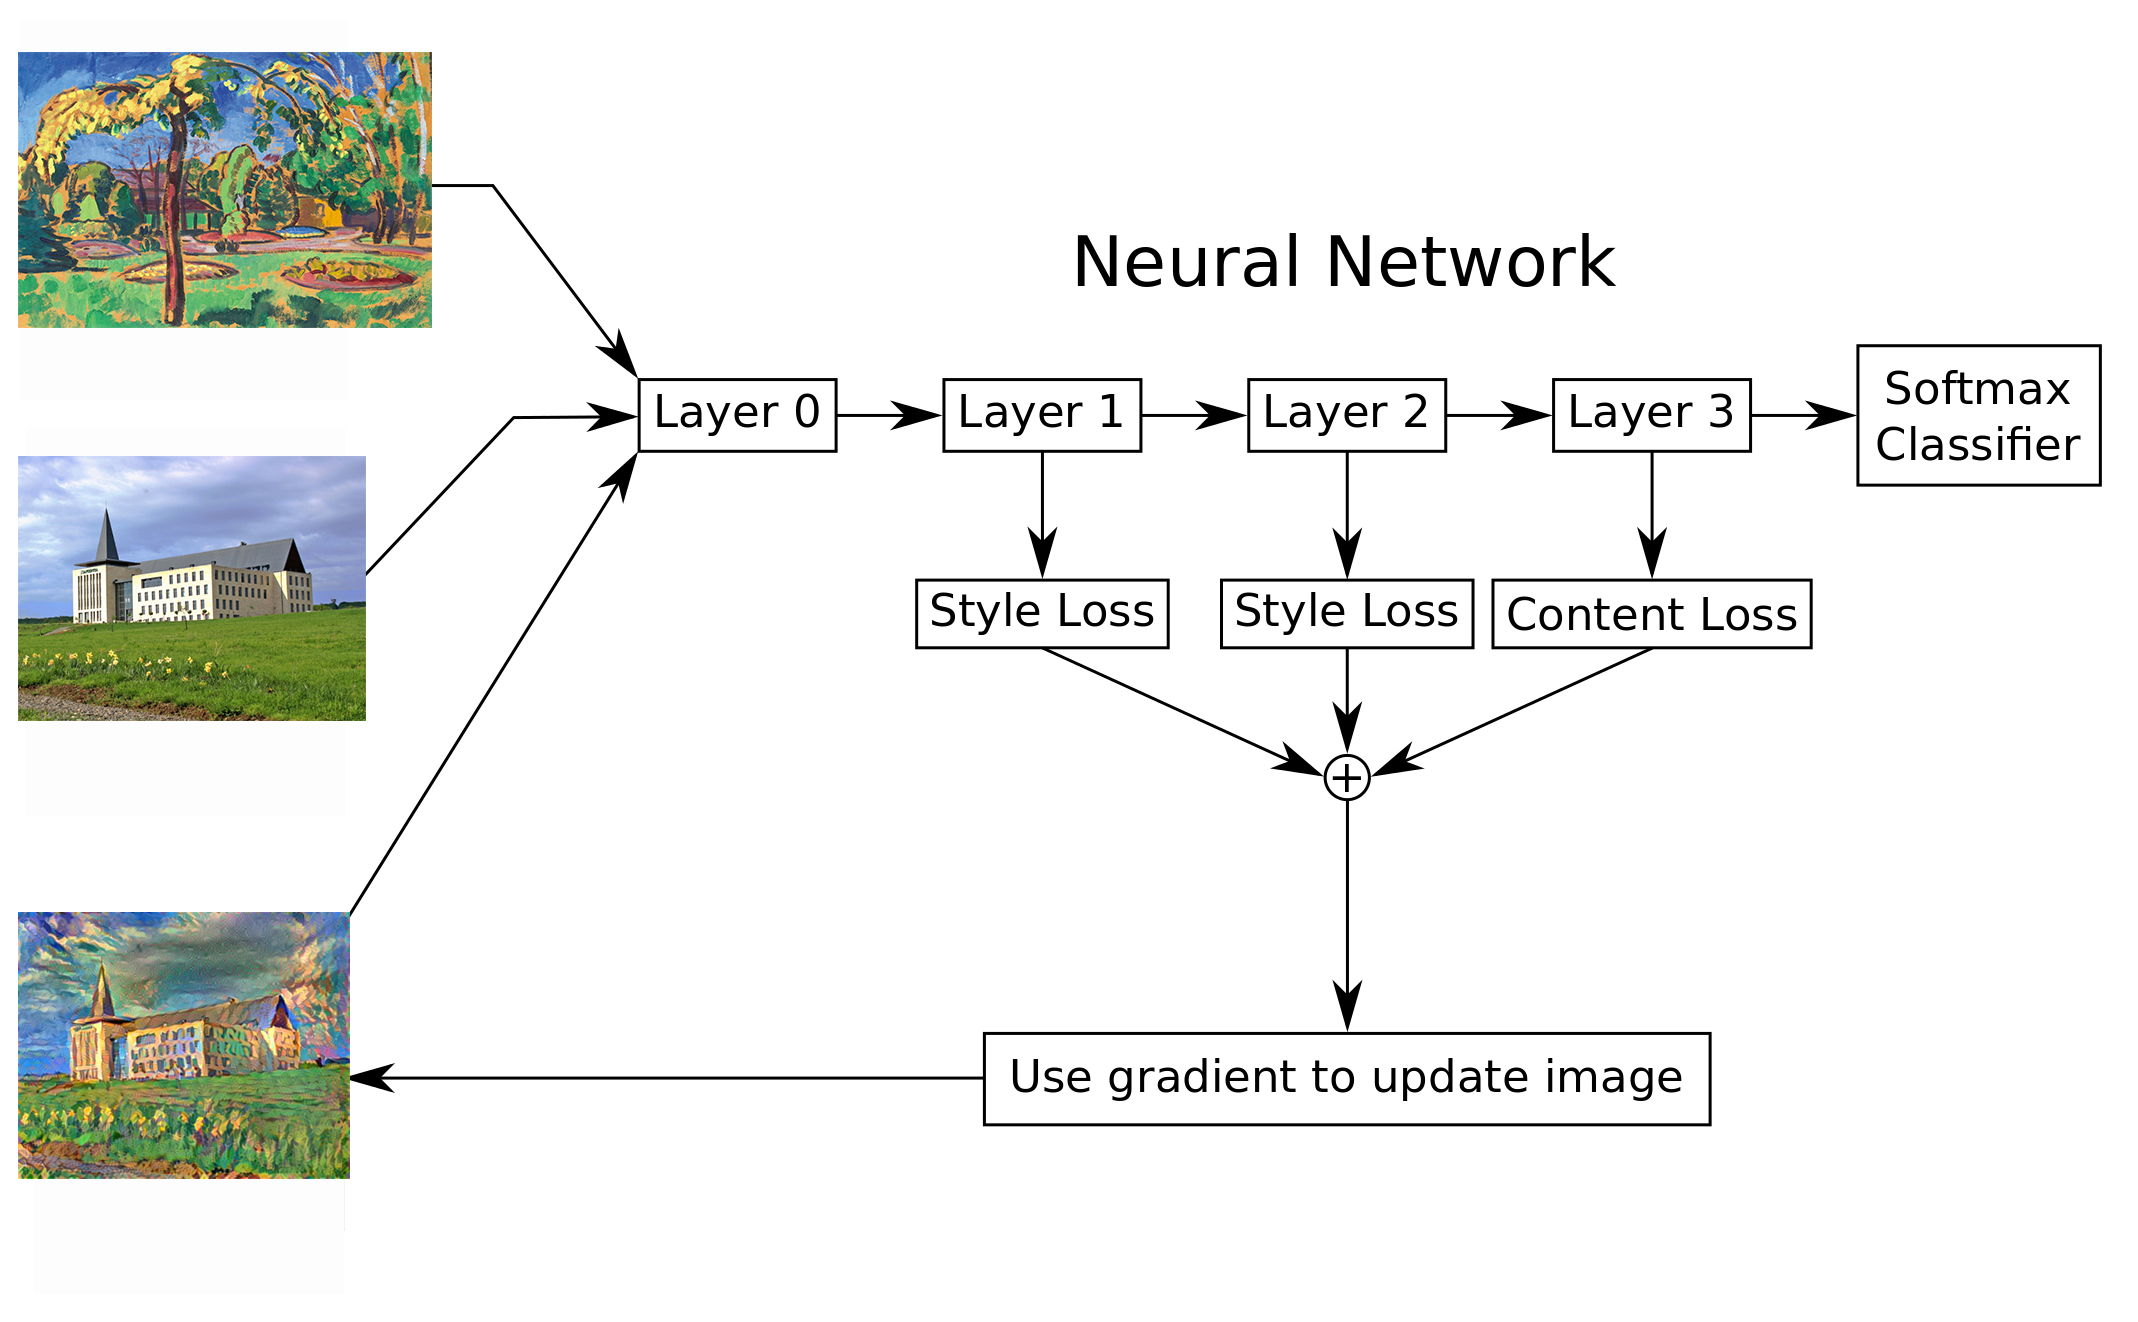
\includegraphics[scale=0.15]{system_presentation.png}
			\end{center}
		\end{figure}
	\end{frame}
	
	\begin{frame}
		\frametitle{A dolgozat célja}
		\begin{itemize}
			\item Grafikus felhasználói felülettel rendelkező alkalmazás fejlesztése 
			\item Gépi tanulást (deep learning) alkalmazó rendszer tervezése és megvalósítása
			\item Híres magyar festők ismertebb műveinek művészeti stílusát átruházni képekre / mozgóképekre
			\item Párhuzamos gépi tanítási folyamat ami kihasználja a GPU által biztosított párhuzamosítási lehetőségeket
		\end{itemize}
	\end{frame}

	\begin{frame}
		\frametitle{A Tensorflow könyvtár bemutatása}
		\begin{center}
			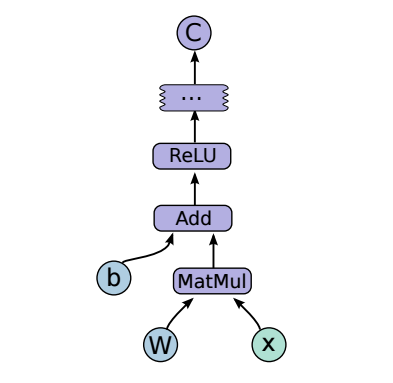
\includegraphics[scale=0.5]{tensorflow_graph.png}
			\captionof{figure}{Tensorflow számítási gráf}
			\source{Google.com}
			\label{tensorflow_graph}
		\end{center}
	\end{frame}

	\begin{frame}
		\frametitle{Párhuzamos tanítás a Tensorflow segítségével}
		\begin{figure}[!htbp]
			\centering
			\subfloat[Adatpárhuzamos megközelítés]{
				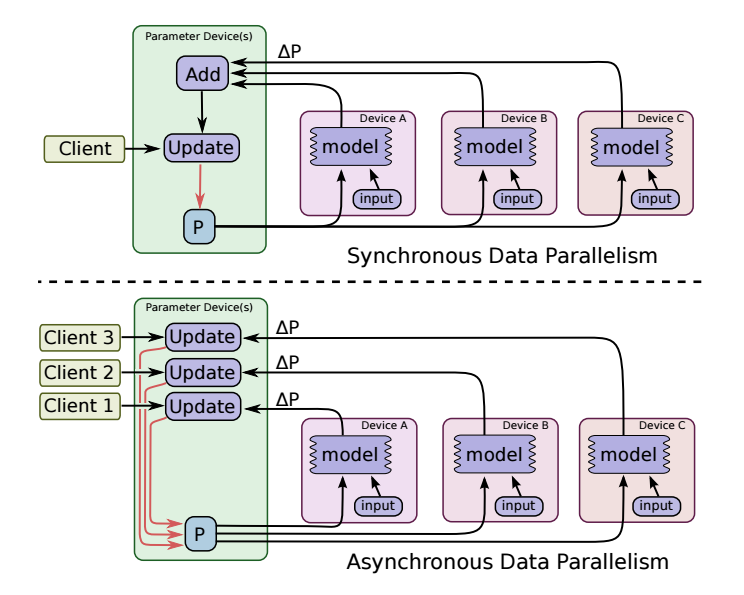
\includegraphics[width=60mm]{data_parallel_tf_model.png}
			}
			\subfloat[Feladatpárhuzamos megközelítés]{
				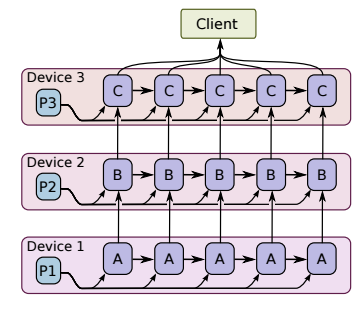
\includegraphics[width=40mm]{task_parallel_tf_model.png}
			}
			\caption{Párhuzamos tanítás}
			\source{Google.com}
		\end{figure}
	\end{frame}

	\section{Megvalósítás}
	
	\begin{frame}
		\frametitle{A rendszer tanítása}
		\begin{itemize}
			\item "Deep learning" tanítási metódus
			\item Előre betanított neuronháló (VGG19: 16 konvolúciós réteg, 5 pooling réteg)
			\item Statikus kép esetében külön tanításra kerül a bemeneti kép és a stílus kép is
			\item Mozgókép esetében minden képkocka tanításra kerül
			\item Temporális összefüggések a képkockák között
		\end{itemize}
	\end{frame}
	
	\begin{frame}
		\frametitle{A tanításhoz használt neuronháló}
		\begin{center}
			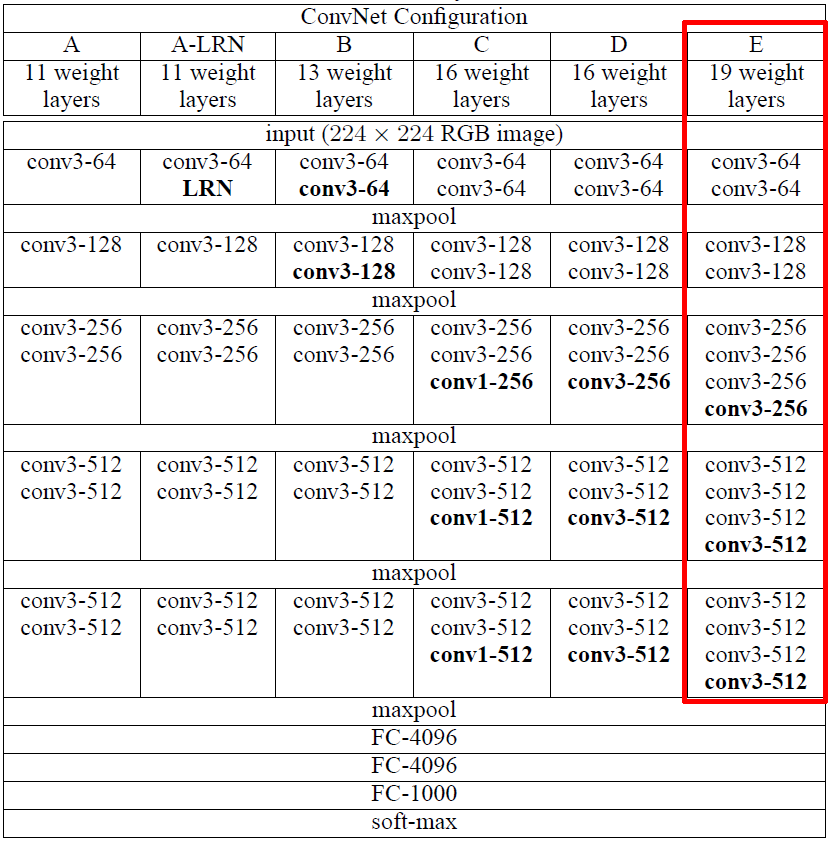
\includegraphics[scale=0.2]{VGG19.png}
			\captionof{figure}{VGG-19 háló szerkezete}
		\end{center}
	\end{frame}

	\begin{frame}
		\frametitle{A bemeneti kép tanítása}
		\begin{itemize}
			\item A konvolúciós szűrök tartalmazzák a kép sajátosságait
			\item Egy adott betanított réteg válasza egy bemeneti képre vizualizálható, ha fehér zaj képre értékeljük ki azt
		\end{itemize}
			
		A bemeneti kép veszteségfüggvénye felírható mint:
		\begin{equation}
			L_{content}(\vec{x}, \vec{r}, l) = \frac{1}{2}\sum{R^l_{ij} - W^l_{ij}}
		\end{equation}
		
		Ahol:
		\begin{itemize}
			\item \(\vec{x}\) - a bemeneti képet
			\item \(R^l\) - az l-edik réteg válasza a bemeneti képre
			\item \(W^l\) - az l-edik réteg válasza a fehér zaj bemenetre
			\item \(\vec{r}\) - pedig azt a kimeneti képet jelenti amit a rendszer generál a rétegek tulajdonságaiból
		\end{itemize}
		
		Kiértékelt réteg: \(conv4\_2\)
	
	\end{frame}

	\begin{frame}
		\frametitle{A stílus kép tanítása}
		\framesubtitle{A Gramm-matrix ismertetése}
		
		\begin{itemize}
			\item A Gramm mátrix egy szorzatot jelen egy adott vektorhalmaz összes elemei között.
			\item Hogyha adott egy vektorhalmazunk \(v_1...v_n\), akkor a \(G\) Gramm mátrixot a következő eljárás szerint határozzuk meg:
				\begin{equation}
					G_{ij} = v_i \cdot v_j
				\end{equation}
			\item A Gramm mátrix \(ij\) pozíciójában elhelyezkedő elem megadja, hogy egy adott réteg \(i\)-dik tulajdonsága mennyire teljesül a \(j\)-dik tulajdonság jelenlétében,
		\end{itemize}
	\end{frame}

	\begin{frame}
		\frametitle{A stílus kép tanítása}
		\framesubtitle{A veszteségfüggvény meghatározása}
		
		Ha az \(l\) rétegnek \(N\) szűrője van, akkor felírható \(G \in R^{N_l*N_l}\) Gramm-mátrix, ahol:
		\begin{equation}
			G^l_{ij} = \sum_{k} F^l_{ik} \cdot F^l_{jk}
		\end{equation}
		
		A veszteségfüggvény egyetlen rétegre felírható mint a fehér zaj kép Gramm mátrixa és a stílus kép Gramm mátrixának átlagos négyzetes hibájaként:
		 
		\begin{equation}
		E_l = \frac{1}{4N^2_l M^2_l} \sum_{i,j} (G_{ij} - A_{lj})^2
		\end{equation}
		
	\end{frame}

	\begin{frame}
		\frametitle{A stilizált kép tisztítása}
		\framesubtitle{Total Variation Denoising}
		
		A stilizált képet és eltoljuk X koordináta mentén egy pixellel, majd az Y koordináta mentén is eltoljuk egy pixellel.
		\begin{equation}
		L_{tv}(\vec{a}, \vec{x}) = \sum_{i,j} \left|(X_{ij} - A_{{i+1}j})\right| + \sum_{i, j} \left|(X_{ij} - A_{i {j+1}})\right|
		\end{equation}
		
	\end{frame}

	\section{A rendszer tesztelese}
	
	\begin{frame}
		\frametitle{A rendszer tesztelese}
	\end{frame}
	
	\section{Osszefoglalo}
	
	\begin{frame}
		\frametitle{Osszefoglalo}
	\end{frame}
	
	
\end{document}